% ---------------------------------------------------------------------------
% PhD defence slides -- Luca Arnaboldi, 26 August 2026.
%
% A re-typeset of slides/draft.key: same 25 slides, same content, same order.
% Every equation that was a screenshot in Keynote is real LaTeX here, and every
% figure is the actual thesis PDF rather than a crop of it.  Presenter notes are
% carried over verbatim as \note.
%
% Build from the REPO ROOT (figure paths are repo-root-relative); the root
% latexmkrc supplies lualatex, -synctex=1 and out_dir=build, so the deck lands
% at build/slides.pdf next to build/thesis.pdf:
%     latexmk -pdflua slides/slides.tex
% ---------------------------------------------------------------------------
\documentclass[aspectratio=169,11pt]{beamer}
% Built from the repo root, so slides-style.sty is not in the CWD; point the
% file search at slides/ rather than duplicating the package at the root.
\makeatletter\def\input@path{{slides/}}\makeatother
\usepackage{slides-style}

\title[Effective Dynamics of SGD]{Effective Dynamics of SGD}
\subtitle{in High-Dimensional Neural Networks}
\author{Luca Arnaboldi}
\institute{EPFL --- IdePHIX}
\date{26 August 2026}

\begin{document}

% === 1. Title ==============================================================
\begin{frame}[plain]
  \begin{columns}[T]
    \begin{column}{0.5\textwidth}
      \begin{center}
        
\includegraphics[height=1.2cm]{slides/figs/logo-epfl}
      \end{center}
    \end{column}
    \begin{column}{0.5\textwidth}
      \begin{center}
        
\includegraphics[height=1.5cm]{slides/figs/logo-idephix}
      \end{center}
    \end{column}
  \end{columns}
  \vfill
  \begin{center}
    {\usebeamercolor[fg]{structure}\Huge\bfseries Effective Dynamics of SGD}\par
    \vspace{0.5em}
    {\LARGE in High-Dimensional Neural Networks}
  \end{center}
  \vfill
  \begin{center}
    \large Luca Arnaboldi \textbar{} PhD Defence \textbar{} 26 August 2026
  \end{center}
  \vspace{1.5em}
\end{frame}

% === 2. Why are we doing this? ==============================================
% draft.key had this as a bare section slide; the two frames here fill it with
% chapters/motivation.tex.  Both pictures are TikZ, so the deck stays
% asset-free (see \aitimeline / \atomprogression in slides-style.sty).
\begin{frame}{Why are we doing this?}
  \begin{center}
    {\Large\bfseries An engineering triumph, seventy years in the making}
  \end{center}
  \vspace{0.4em}
  \aitimeline
  \vspace{0.4em}
  \punchline{We can train these models. We still cannot say \emph{why} they work.}
  \vspace{0.8em}
  \begin{columns}[t]
    \begin{column}{0.31\textwidth}\centering
      \role{\large Practical}\par\vspace{0.35em}
      \small better algorithms, more efficient models, less compute and energy
      burnt
    \end{column}
    \begin{column}{0.31\textwidth}\centering
      \role{\large Social}\par\vspace{0.35em}
      \small interpretability, fairness, robustness --- the prerequisites for
      high-stakes deployment
    \end{column}
    \begin{column}{0.31\textwidth}\centering
      \role{\large Scientific}\par\vspace{0.35em}
      \small this thesis goes to the \emph{\'Ecole Doctorale de Physique}:
      understanding a complex system is a goal in itself
    \end{column}
  \end{columns}
  \note{The release of ChatGPT made public something that had been building in
    the labs for years, and it was above all an engineering achievement: a
    pipeline able to digest essentially all of human digital knowledge.
    Decades of cumulative work -- artificial neurons in the 50s,
    backpropagation in the 80s, GPUs and large datasets in the 2000s and 2010s.
    But the theory did not keep up.
    Three reasons to close the gap: practical, social, and -- since we are
    physicists -- plain curiosity, which historically pays off in unexpected
    ways.}
\end{frame}

% === 3. What does a physicist do about it? ==================================
\begin{frame}{What does a physicist do about it?}
  \begin{columns}[T]
    \begin{column}{0.55\textwidth}
      \role{\large Why the classical theory does not apply}
      \begin{itemize}
        \setlength{\itemsep}{0.35em}
        \item fitting data with a huge number of parameters breaks the
          bias--variance trade-off
        \item non-convex landscape, no closed-form solution
        \item \dots\ yet plain SGD finds solutions that generalize
      \end{itemize}
      \vspace{0.9em}
      \role{\large So we build a caricature}\par\vspace{0.25em}
      \small Simplified and certainly incomplete, but \emph{concrete enough} to be
      tested, refuted and improved.
    \end{column}
    \begin{column}{0.45\textwidth}
      \centering
      \atomprogression
    \end{column}
  \end{columns}
  \vspace{0.4em}
  \punchline{We want to be Thomson, so that someone can be Bohr after us.}
  \vspace{0.6em}
  \begin{columns}[t]
    \begin{column}{0.5\textwidth}\centering\small
      \role{Worst case} \aside{(PAC, VC, Rademacher)}\par
      $\longrightarrow$ pessimistic bounds
    \end{column}
    \begin{column}{0.5\textwidth}\centering\small
      \role{Typical case} \aside{(statistical physics)}\par
      $\longrightarrow$ sharp predictions
    \end{column}
  \end{columns}
  \note{Chemistry at the end of the nineteenth century could synthesize
    complex molecules without knowing why atoms bond: Thomson's model was crude
    and wrong in important ways, but concrete enough to be improved into Bohr,
    and eventually into quantum mechanics.  That is roughly where deep learning
    stands, and the role we aspire to play.
    Two advantages we have: the experiments run on a laptop rather than a
    collider, and the process itself -- training -- is mathematically well
    defined, so we only need to explain \emph{why} it works and \emph{how} the
    dynamics unfold.
    Last line: this is why we use statistical physics rather than classical
    learning theory, and the thread of the thesis is the typical dynamics of
    SGD in high dimension.}
\end{frame}

% === 4. Our setting =========================================================
\begin{frame}{Our setting}
  \begin{center}
    {\Large\bfseries Supervised Learning with scalar labels}
  \end{center}
  \vspace{0.3em}
  \begin{center}
    \small
    $\mathcal{D} = \{(\vec{x}^\nu,\, y^\nu)\}_{\nu \in [n]}$ i.i.d.,\quad
    $\vec{x} \in \mathbb{R}^d$ ($d \gg 1$),\quad $y \in \mathbb{R}$
    \quad$\longrightarrow$\quad
    find $f$ with $f(\vec{x}) \approx y$ on \emph{unseen} data
  \end{center}
  % \vspace{0.1em}
  \begin{center}
    \aside{The most controlled paradigm there is --- and a scalar label carries
      more signal than a class label.}
  \end{center}
  % \vspace{0.25em}
  \begin{center}
    \large We need to make some assumptions for our theory on 
  \end{center}
  \vspace{0.4em}
  \begin{columns}[t]
    \begin{column}{0.33\textwidth}\centering
      \icondata\par\vspace{0.25em}
      \role{\large The data}\par\vspace{0.2em}
      % \small Where do the inputs come from, and how is the label built?
    \end{column}
    \begin{column}{0.33\textwidth}\centering
      \iconmodel\par\vspace{0.25em}
      \role{\large The model}\par\vspace{0.2em}
      % \small Which family of functions do we fit, and how do we score it?
    \end{column}
    \begin{column}{0.33\textwidth}\centering
      \iconalgo\par\vspace{0.25em}
      \role{\large The algorithm}\par\vspace{0.2em}
      % \small How are the parameters updated, and with how much data?
    \end{column}
  \end{columns}
  \vspace{1.2em}
  \punchline{Keep only what the phenomenon needs, strip everything else.}
  \note{This is not of course our idea. It has been build on ton of literature.
    We are based on 3 pillars.
  }
\end{frame}

% === 5. The multi-index models =============================================
\begin{frame}{The multi-index models}
  \begin{columns}[T]
    \begin{column}{0.50\textwidth}
      \role{\large Gaussian data}
      \vspace{-0.4em}
      \[ \vec{x} \sim \mathcal{N}(0, I_d) \]

      \role{\large The target function}
      \vspace{-0.4em}
      \[ f^\star(\vec{x}) = h^\star\!\left(\frac{W^\star \vec{x}}{\sqrt{d}}\right) \]
      \vspace{-1.0em}
      \begin{center}
        \small
        $h^\star : \mathbb{R}^k \to \mathbb{R}$,\qquad
        $W^\star = \{\vec{w}^\star_r\}_{r \in [k]} \in \mathbb{R}^{k \times d}$
        % \par\vspace{0.25em}
        % \aside{we call $f^\star$ the \emph{teacher}}\par
        % \aside{$k = \mathcal{O}(1) \ll d$;\;
        %   $k = 1$ is the \emph{single-index} model}
      \end{center}
      \vspace{0.2em}

      \role{\large (Possible) label noise}
      % \vspace{-0.4em}
      \[
        y = f^\star(\vec{x}) + \sqrt{\Delta}\,\xi,
        \qquad \xi \sim \mathcal{N}(0,1)
      \]
    \end{column}
    \begin{column}{0.50\textwidth}
      \centering
      \thesisnet[0.82\linewidth]{chapters/figs/multi-index.tex}
      \vspace{-1.0em}
      \begin{defbox}{Teacher subspace}
        \centering
        $V^\star = \operatorname{span}(\vec{w}^\star_1, \ldots, \vec{w}^\star_k)$,
        \qquad $\dim V^\star = k \ll d$
        \vspace{0.15em}

        \emph{Learning $\equiv$ discovering $V^\star$}
      \end{defbox}
    \end{column}
  \end{columns}
  \vspace{1.2em}
  \punchline{These $k$ directions \emph{are} the features of the problem.}
  \note{$d$ is going to be be big, while $k$ is small and fixed: discovering the
    subspace $W^\star$ is actually a proxy of feature learning.\\
    We call this teacher.}
\end{frame}

% === 6. The learned model: 2-layer network =================================
\begin{frame}{The learned model: 2-layer network}
  \begin{columns}[c]
    \begin{column}{0.52\textwidth}
      \[
        f(\vec{x};\, W, \vec{a})
        = \frac{1}{p} \sum_{j=1}^p a_j\,
          \sigma\!\left(\frac{\langle \vec{w}_j, \vec{x}\rangle}{\sqrt{d}}\right)
      \]
    \end{column}
    \begin{column}{0.48\textwidth}
      \centering
      \thesisnet[0.95\linewidth]{chapters/figs/two-layer-net.tex}
    \end{column}
  \end{columns}
  \vspace{0.3em}
  \punchline{The student is a \emph{special case} of the teacher, and it is a \emph{two-layer NN}.}
  \vspace{0.5em}
  \begin{columns}[t]
    \begin{column}{0.42\textwidth}
      \centering
      \role{\large Loss function}
      \[ \ell(\hat{y}, y) = \tfrac{1}{2}(\hat{y} - y)^2 \]
    \end{column}
    \begin{column}{0.58\textwidth}
      \centering
      \role{\large Population risk}
      \[
        \mathcal{R}(W, \vec{a}) = \mathbb{E}_{(\vec{x},\, y)}\!\left[
          \tfrac{1}{2}\bigl(f(\vec{x};\, W, \vec{a}) - y\bigr)^2\right]
      \]
    \end{column}
  \end{columns}
  \note{$W$, $\vec{a}$ are the weights. $\sigma$ is the activation function.
    We need to align the student subspace with the teacher one to get good learning.
    This is the natural loss for regression.
    The population risk then is the best measure of the performance, but of
    course it can't be used for training (otherwise we have an equivalent of
    data leakage).}
\end{frame}

% === 7. The algorithm: one-pass SGD ========================================
\begin{frame}{The algorithm: one-pass SGD}
  \begin{columns}[c]
    \begin{column}{0.26\textwidth}\raggedleft\role{\large Update}\end{column}
    \begin{column}{0.74\textwidth}
      \[
        \vec{w}_j^{\,\nu+1} = \vec{w}_j^{\,\nu}
          - \gamma\,\nabla_{\vec{w}_j}\,
            \ell\!\left(f(\vec{x}^\nu;\, W^\nu, \vec{a}),\, y^\nu\right),
        \qquad j \in [p],
      \]
    \end{column}
  \end{columns}
  \vspace{-0.3em}
  \begin{center}
    \aside{$\gamma > 0$ is the \emph{learning rate}; each step draws a
      \emph{fresh} sample, uses it once, and never reuses it}
  \end{center}
  \vspace{0.8em}
  \begin{columns}[c]
    \begin{column}{0.26\textwidth}\raggedleft\role{\large Initialization}\end{column}
    \begin{column}{0.74\textwidth}
      \[ \vec{w}_j^0 \sim \mathcal{N}(0, I_d) \]
    \end{column}
  \end{columns}
  \vspace{0.8em}
  \begin{columns}[c]
    \begin{column}{0.26\textwidth}\raggedleft\role{\large Steps $=$ samples}\end{column}
    \begin{column}{0.74\textwidth}
      After $n$ steps the algorithm has consumed exactly $n$ samples: counting
      steps \emph{is} counting samples.
    \end{column}
  \end{columns}
  \vspace{0.8em}
  \begin{columns}[c]
    \begin{column}{0.26\textwidth}\raggedleft\role{\large The key property}\end{column}
    \begin{column}{0.74\textwidth}
      \punchline{Independence of the steps}
    \end{column}
  \end{columns}
  \vfill
  \begin{center}
    \aside{We actually often consider a spherical constrained dynamics for
      simplicity:}\quad
      
      \vspace{0.7em }
    $\displaystyle \vec{w}^{\nu+1} = \sqrt{d}\,
      \frac{\vec{w}^\nu - \gamma\nabla_{\vec{w}}\ell(f(\vec{x}^\nu), y^\nu)}
           {\bigl\lVert \vec{w}^\nu
             - \gamma\nabla_{\vec{w}}\ell(f(\vec{x}^\nu), y^\nu)\bigr\rVert}$
  \end{center}
  \note{$W$, $\vec{a}$ are the weights. $\sigma$ is the activation function.
    It is one pass because every sample is used once then discarded forever.
    That also means the number of steps and the number of samples are the same
    number, so from here on the sample complexity of a problem is just how long
    the dynamics has to run -- which is what the second half of the talk
    counts.}
\end{frame}

% === 8. The reduced dynamic ================================================
% Three bands, top to bottom: the projections both networks see, the order
% parameters that fix their joint law, the risk that follows.  The order
% parameters get the green definition box -- they are the object the rest of
% the talk is written in -- rather than being squeezed onto one \fiteq line
% with the covariance.
\begin{frame}{The reduced dynamic}
  \begin{columns}[c]
    \begin{column}{0.27\textwidth}
      \raggedleft
      \role{\large Pre-activations are Gaussian}
    \end{column}
    \begin{column}{0.73\textwidth}
      \[
        \vec{\lambda} = \frac{W \vec{x}}{\sqrt{d}} \in \mathbb{R}^p,
        \qquad
        \vec{\lambda}^\star = \frac{W^\star \vec{x}}{\sqrt{d}} \in \mathbb{R}^k
      \]
      \vspace{-0.7em}
      \[
        f(\vec{x};\, W, \vec{a}) = h(\vec{\lambda}, \vec{a}),
        \qquad
        h(\vec{\lambda}, \vec{a}) = \frac{1}{p}\sum_{j=1}^p a_j\,\sigma(\lambda_j)
      \]
    \end{column}
  \end{columns}
  \vspace{0.2em}
  \begin{defbox}[top=3pt, bottom=2pt]{Sufficient low-dimensional statistics}
    \fiteq{
      Q_{jl} = \frac{\langle \vec{w}_j, \vec{w}_l\rangle}{d}, \qquad
      M_{jr} = \frac{\langle \vec{w}_j, \vec{w}^\star_r\rangle}{d}, \qquad
      P_{rs} = \frac{\langle \vec{w}^\star_r, \vec{w}^\star_s\rangle}{d}}
    \fiteq{
      (\vec{\lambda}, \vec{\lambda}^\star) \sim \mathcal{N}(0, \Omega),
      \qquad
      \Omega = \begin{pmatrix} Q & M \\ M^\top & P \end{pmatrix}
        \in \mathbb{R}^{(p+k) \times (p+k)}}
  \end{defbox}
  \vspace{0.2em}
  \begin{columns}[c]
    \begin{column}{0.27\textwidth}
      \raggedleft
      \role{\large Population risk is $d$-independent}
    \end{column}
    \begin{column}{0.73\textwidth}
      \[
        \mathcal{R}(\Omega, \vec{a})
        = \mathbb{E}_{(\vec{\lambda}, \vec{\lambda}^\star) \sim \mathcal{N}(0, \Omega)}
          \!\left[\tfrac{1}{2}
            \bigl(h(\vec{\lambda}, \vec{a}) - h^\star(\vec{\lambda}^\star)\bigr)^2\right]
      \]
    \end{column}
  \end{columns}
  \note{Low dimensional aka independent of $d$.}
\end{frame}

% === 9. The reduced dynamic: update rule ===================================
% Laid out as a four-row grid with a fixed arrow gutter at 0.40/0.06/0.54: the
% left column is everything in weight space, the right column the same object
% in statistics space.  The old prose correspondence block ("update rule for
% $W$ $\leftrightarrow$ update rule for $(Q,M,\vec a)$") is gone -- the grid
% says it -- and its two remaining lines became rows 3 and 4.
% The $\lVert\vec x^\nu\rVert^2/d$ term is tinted to match the asterisk in the
% headline: it is the one thing that is not exactly self-closed, and it
% concentrates to 1 in high dimension.  Spoken, not written.
\begin{frame}{The reduced dynamic: update rule}
  \begin{center}\large
    Update rule is self-closed too!{\color{slideorange}*}
  \end{center}
  \vspace{0.2em}
  \begin{columns}[c]
    \begin{column}{0.40\textwidth}
      \centering\role{\large In the weights}
    \end{column}
    \begin{column}{0.06\textwidth}\end{column}
    \begin{column}{0.54\textwidth}
      \centering\role{\large In the sufficient statistics}
    \end{column}
  \end{columns}
  \vspace{0.2em}
  \begin{columns}[c]
    \begin{column}{0.40\textwidth}
      \fiteq{
        \begin{aligned}
          \vec{w}_j^{\nu+1} &= \vec{w}_j^{\nu}
            + \frac{\gamma}{p\sqrt{d}}
              \left( y^\nu(\vec{\lambda}^{\star,\nu}) - h(\vec{\lambda}^{\nu}) \right)
              a_j \sigma'(\lambda^\nu_j) \vec{x}^\nu, \\
          a_j^{\nu+1} &= a_j^{\nu}
            + \frac{\gamma}{pd}
              \left( y^\nu(\vec{\lambda}^{\star,\nu}) - h(\vec{\lambda}^{\nu}) \right)
              \sigma(\lambda^\nu_j)
        \end{aligned}}
    \end{column}
    \begin{column}{0.06\textwidth}
      \centering$\Longrightarrow$
    \end{column}
    \begin{column}{0.54\textwidth}
      \fiteq{
        \begin{aligned}
          Q^{\nu+1}_{jl} =\;& Q^{\nu}_{jl}
            + \frac{\gamma}{pd}
              \left( y^\nu(\vec{\lambda}^{\star,\nu}) - h(\vec{\lambda}^{\nu}) \right)
              \left( a_l \sigma'(\lambda^\nu_l) \lambda^\nu_j
                   + a_j \sigma'(\lambda^\nu_j) \lambda^\nu_l \right) + \\
            &+ \frac{\gamma}{pd}\frac{\gamma}{p}
              \left( y^\nu(\vec{\lambda}^{\star,\nu}) - h(\vec{\lambda}^{\nu}) \right)^2
              a_j a_l \sigma'(\lambda^\nu_j) \sigma'(\lambda^\nu_l)
              {\color{slideorange}\frac{\lVert\vec{x}^\nu\rVert^2}{d}}, \\
          M^{\nu+1}_{jr} =\;& M^{\nu}_{jr}
            + \frac{\gamma}{pd}
              \left( y^\nu(\vec{\lambda}^{\star,\nu}) - h(\vec{\lambda}^{\nu}) \right)
              a_j \sigma'(\lambda^\nu_j) \lambda^{\star,\nu}_r, \\
          a_j^{\nu+1} =\;& a_j^{\nu}
            + \frac{\gamma}{pd}
              \left( y^\nu(\vec{\lambda}^{\star,\nu}) - h(\vec{\lambda}^{\nu}) \right)
              \sigma(\lambda^\nu_j).
        \end{aligned}}
    \end{column}
  \end{columns}
  \vspace{0.4em}
  \begin{columns}[c]
    \begin{column}{0.40\textwidth}
      \centering
      sample $\vec{x}^\nu \sim \mathcal{N}(0, I_d)$
    \end{column}
    \begin{column}{0.06\textwidth}
      \centering$\Longrightarrow$
    \end{column}
    \begin{column}{0.54\textwidth}
      \centering
      sample $(\vec{\lambda}^\nu, \vec{\lambda}^{\star,\nu}) \sim \mathcal{N}(0, \Omega)$
    \end{column}
  \end{columns}
  \vspace{0.3em}
  \begin{columns}[c]
    \begin{column}{0.40\textwidth}
      \centering
      population risk $\mathcal{R}(W)$
    \end{column}
    \begin{column}{0.06\textwidth}
      \centering$\Longrightarrow$
    \end{column}
    \begin{column}{0.54\textwidth}
      \centering
      population risk $\mathcal{R}(Q, M, \vec{a})$
    \end{column}
  \end{columns}
  \vspace{2em}
  \punchline{There is no need to work with $W$, let's look at $Q,M,P$}
  \note{Low dimensional aka independent of $d$.}
\end{frame}

% === 10. The magic of high-dimensional data =================================
% Split out of the old single frame, which crushed the plateau figures to a
% quarter width and the ODEs to a six-line \fiteq.  This half carries the
% equations only, written in the compact form frame 16 already uses
% (dQ/dt = Phi + gamma/p Psi) with the four expectations demoted to a
% definition box, rather than the thesis's inline over/underbrace form.
\begin{frame}{The magic of high-dimensional data}
  \begin{center}
    \large The stochastic process concentrates into a set of ODEs!
    \quad\cit{Saad \& Solla, 1995}
  \end{center}
  \vspace{0.1em}
  \begin{columns}[c]
    \begin{column}{0.56\textwidth}
      \[
        \begin{aligned}
          \frac{\dd Q_{jl}}{\dd t} &= \Phi^{Q}_{jl}(\Omega, \vec{a})
            + \frac{\gamma}{p}\,\Psi^{Q}_{jl}(\Omega, \vec{a}), \\[0.2em]
          \frac{\dd M_{jr}}{\dd t} &= \Phi^{M}_{jr}(\Omega, \vec{a}), \\[0.2em]
          \frac{\dd a_{j}}{\dd t} &= \Phi^{a}_{j}(\Omega, \vec{a}).
        \end{aligned}
      \]
    \end{column}
    \begin{column}{0.44\textwidth}
      \centering
      \role{\large The time-step}
      \[ \delta t = \frac{\gamma}{pd} \]
      \vspace{-0.6em}
      \par
      \aside{infinitesimal in high dimension:
        $\nu \longmapsto t = \nu\,\dfrac{\gamma}{pd}$}
    \end{column}
  \end{columns}
  \vspace{0.15em}
  \begin{defbox}[top=3pt, bottom=2pt]{Drift $\Phi$ and noise $\Psi$
      \titleaside{expectation over
        $(\vec{\lambda}, \vec{\lambda}^\star) \sim \mathcal{N}(0, \Omega)$}}
    \fiteq{
      \begin{aligned}
        \Phi^{Q}_{jl} &= \mathbb{E}\left[
          \left( h^\star(\vec{\lambda}^{\star}) - h(\vec{\lambda}) \right)
          \left( a_l \sigma'(\lambda_l) \lambda_j
               + a_j \sigma'(\lambda_j) \lambda_l \right)\right],
        &\qquad
        \Phi^{M}_{jr} &= \mathbb{E}\left[
          \left( h^\star(\vec{\lambda}^{\star}) - h(\vec{\lambda}) \right)
          a_j \sigma'(\lambda_j) \lambda^{\star}_r \right], \\[0.3em]
        \Psi^{Q}_{jl} &= \mathbb{E}\left[
          \left(\left( h^\star(\vec{\lambda}^{\star}) - h(\vec{\lambda}) \right)^2
            + \Delta\right) a_j a_l \sigma'(\lambda_j) \sigma'(\lambda_l) \right],
        &\qquad
        \Phi^{a}_{j} &= \mathbb{E}\left[
          \left( h^\star(\vec{\lambda}^{\star}) - h(\vec{\lambda}) \right)
          \sigma(\lambda_j) \right].
      \end{aligned}}
  \end{defbox}
  \note{This is an intuition: LHT gets closer and closer to a derivative, while
    the RHS s some sort of thermodynamic limit (this is the closest I can get to
    physics in this presentation).
    A bit of taxonomy of the SS equations: one term is the drift (gradient flow
    for the population risk), while the other is an high-dimensional noise term
    that survive the limit: it is distinguishing characteristics of SS dynamic!}
\end{frame}

% === 11. The ODEs are exact in high dimension ==============================
% Second half of the old frame 10: the plateau figures at a size one can
% actually read from the back of the room, and the concentration bound as a
% theorem box (orange, the deck's theorem colour) with its source.
\begin{frame}{The ODEs are exact in high dimension}
  \begin{columns}[T]
    \begin{column}{0.5\textwidth}
      \centering
      \includegraphics[height=0.43\textheight]%
        {chapters/figs/saad-solla-plateau/plateau-noiseless}
      \par\vspace{0.15em}
      \aside{$\Delta = 0$: the excess risk falls to zero}
    \end{column}
    \begin{column}{0.5\textwidth}
      \centering
      \includegraphics[height=0.43\textheight]%
        {chapters/figs/saad-solla-plateau/plateau-noisy}
      \par\vspace{0.15em}
      \aside{$\Delta = 10^{-3}$: the noise term $\Psi$ pins a plateau}
    \end{column}
  \end{columns}
  \vspace{0.4em}
  \begin{thmbox}[top=3pt, bottom=2pt]{The actual bound
      \titlecit{Goldt, Advani, Saxe, Krzakala \& Zdeborov\'a, 2019}}
    \fiteq{
      \max_{0 \le \nu \le Td} \mathbb{E}\left[
        \left\lVert (\Omega^\nu, \vec{a}^\nu)
          - \left(\tilde{\Omega}\!\left(\frac{\nu\gamma}{pd}\right),
                  \tilde{\vec{a}}\!\left(\frac{\nu\gamma}{pd}\right)\right)
        \right\rVert \right] \le \frac{C(T)}{\sqrt{d}}}
  \end{thmbox}
  \note{Those are erf--erf plots, the classic of committee machines.}
\end{frame}

% === 12. Other limits, same equations ======================================
% No frame title in draft.key: the delta-t line doubles as the heading -- which
% also frees the whole text height for the triangle, the one thing this frame
% is about.  Everything else is a caption to it: the transition line above, the
% surviving-drift note below.  First frame of the author's own work, hence the
% chapter tag.
\begin{frame}
  \chaptertag{Chapter 2}
  % No frame title here, so the first line would run straight under the tag.
  \vspace*{1.1em}
  \begin{center}
    $\displaystyle \delta t = \frac{\gamma}{pd}$\quad
    {\large d to infinity is only a third of the story though\ldots}
    \quad\cit{Veiga et al., 2022}
  \end{center}
  \punchline{We can have other limits leading to the same equations!}
  \begin{center}
    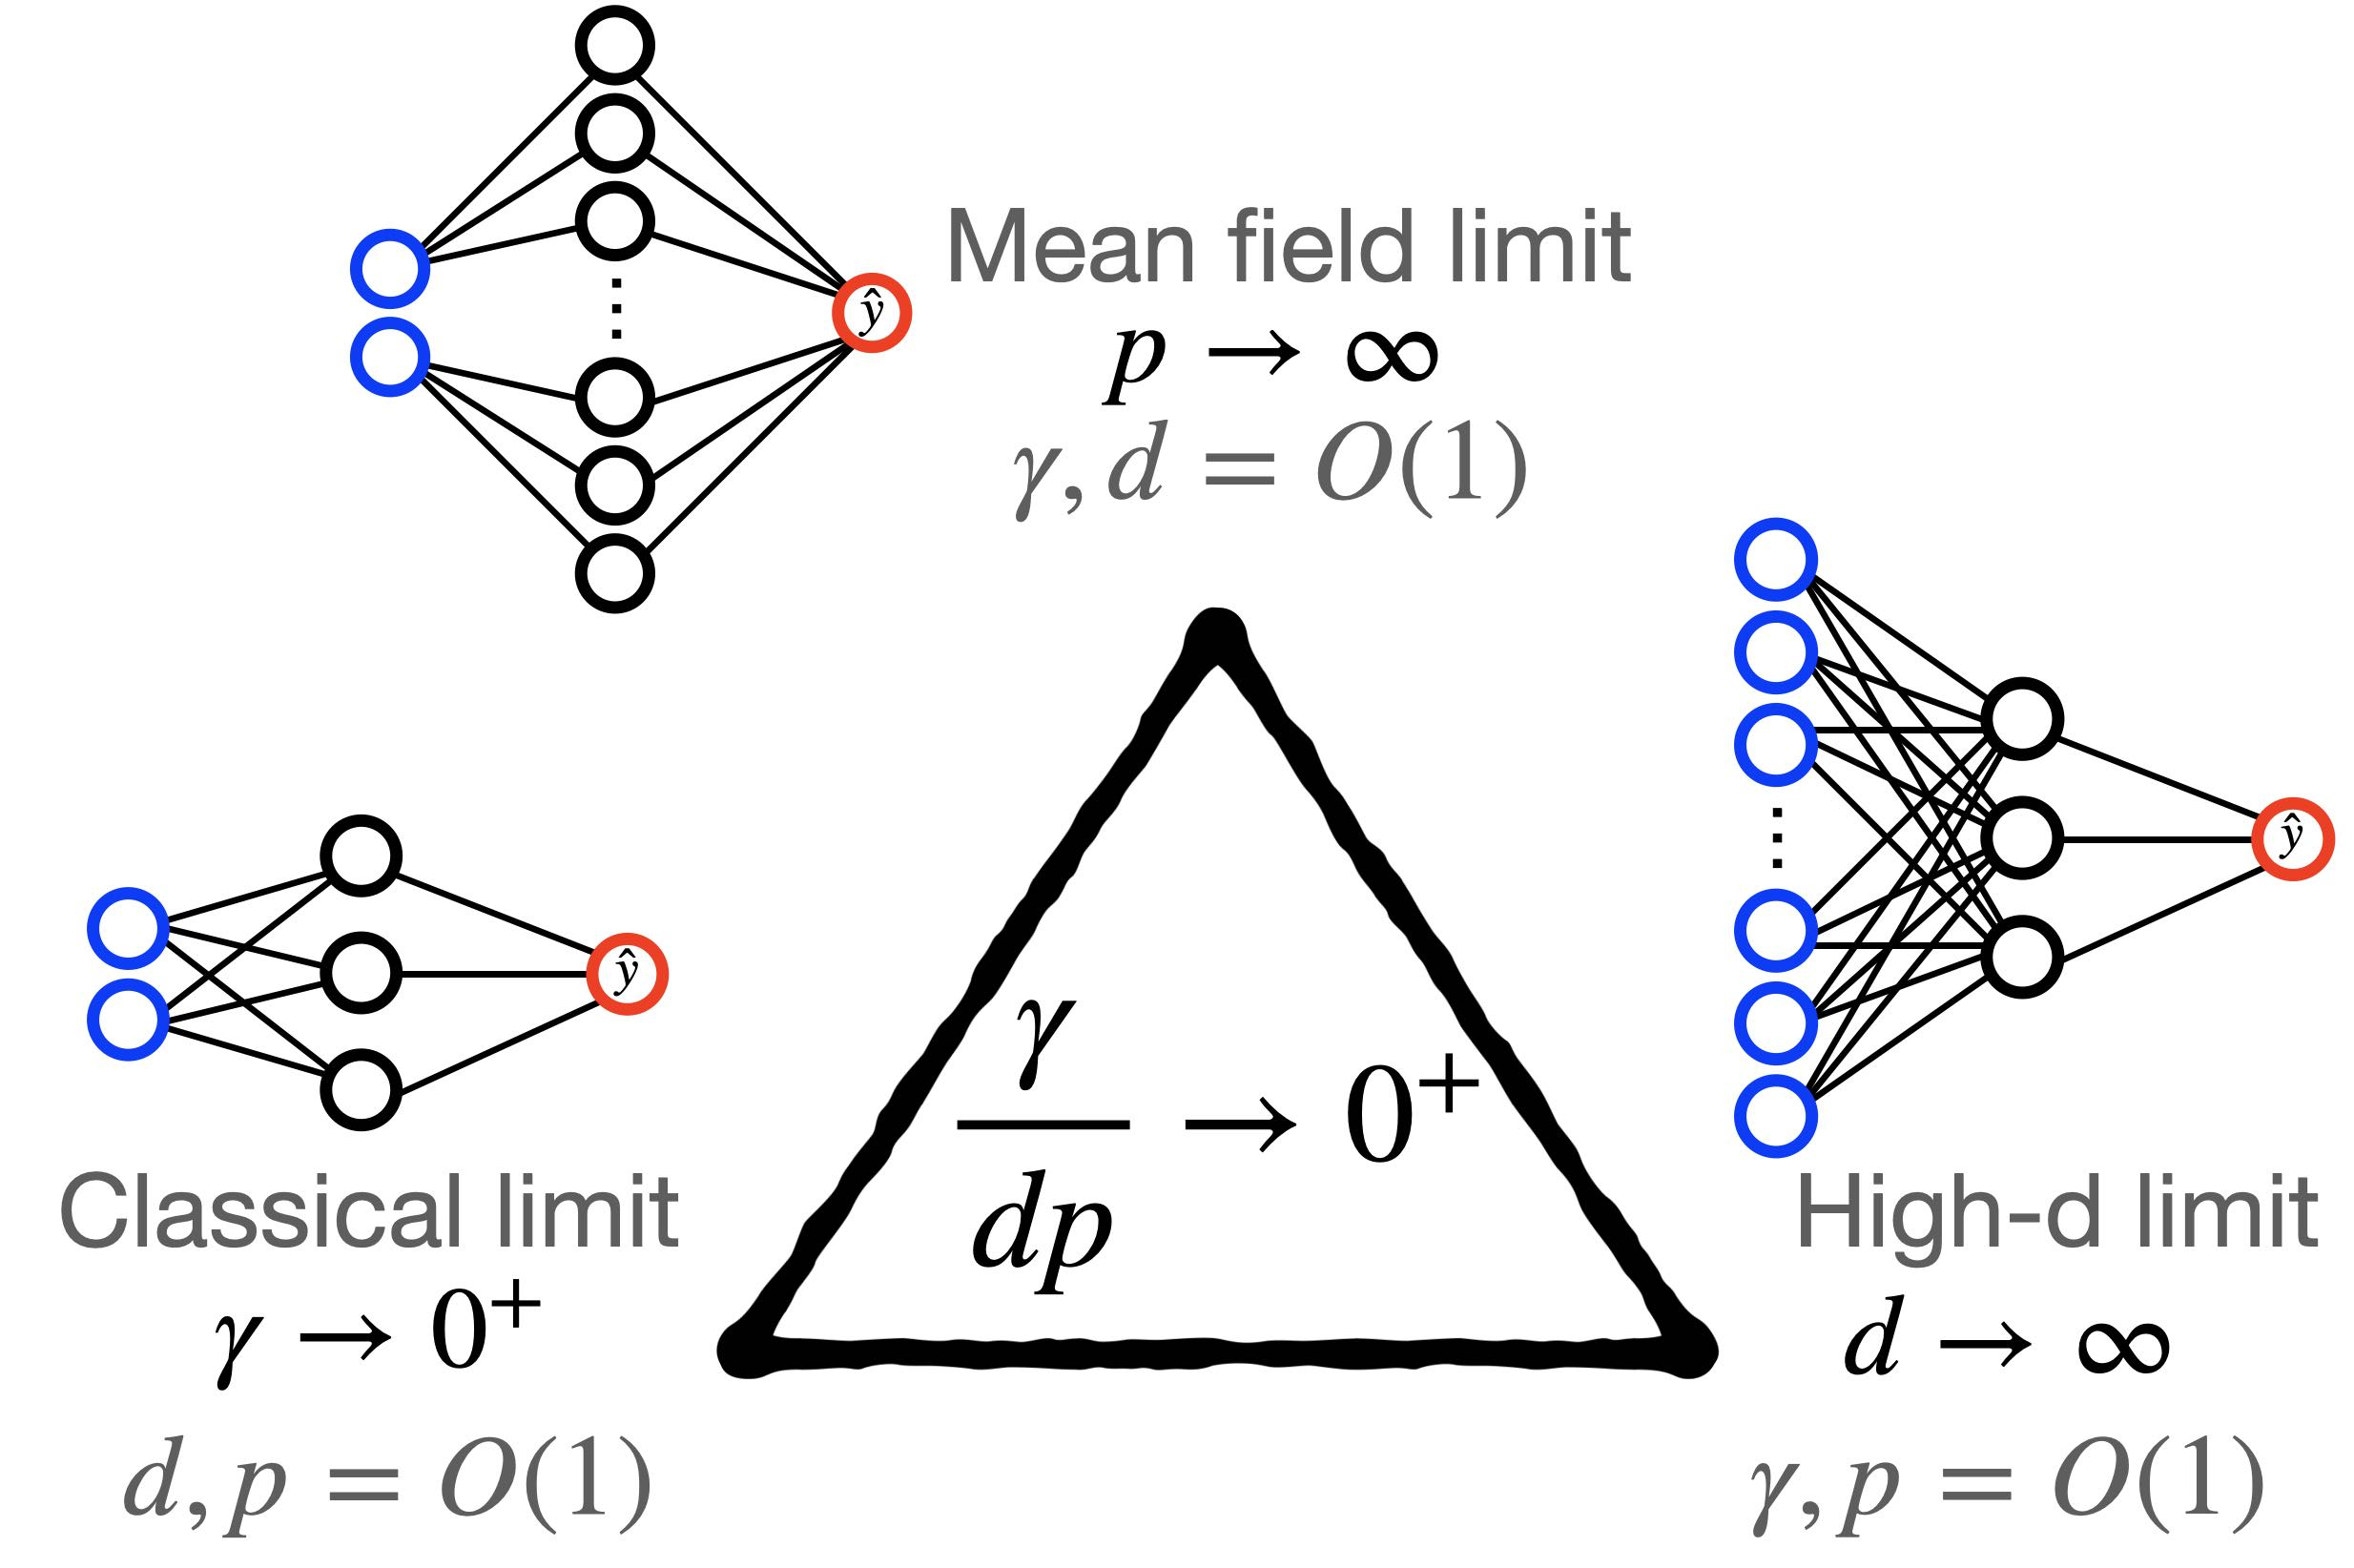
\includegraphics[height=0.60\textheight]{papers/2302/figs/TriangleV3}
  \end{center}
  \begin{center}
    \aside{Only the drift survives in other limits:}\quad
    {\small $\dd Q/\dd t = \Phi^Q
      + {\color{black!35}(\gamma/p)\,\Psi^Q}$}
  \end{center}
\end{frame}

% === 13. Classical limit: gradient flow ====================================
\begin{frame}{Classical limit: gradient flow}
  \chaptertag{Chapter 2}
  \vspace{-0.5em}
  \begin{center}
    \aside{$\gamma \to 0^+$ at fixed $d,\, p = \mathcal{O}(1)$}
  \end{center}
  \vspace{0.2em}
  \begin{columns}[c]
    \begin{column}{0.44\textwidth}
      \centering
      \includegraphics[height=0.54\textheight]%
        {papers/2302/figs/classic/classic_limit_d_plot_-k5_p10_noise0.001_gamma0.0500}
      \par\vspace{0.1em}
      \aside{same initial condition, $d = 5,\,10,\,50$}
    \end{column}
    \begin{column}{0.56\textwidth}
      \centering
      \role{Gradient flow on the weights}\;
      \cit{Robbins \& Monro, 1951}
      \begin{equation*}
        \frac{\dd \vec{w}_j(t)}{\dd t}
          = -\nabla_{\vec{w}_j}\mathcal{R}\bigl(W(t)\bigr)
        \tag*{\aside{$p(d+1)$ parameters}}
      \end{equation*}
      \vspace{-0.7em}
      $\Big\downarrow$\; \aside{chain rule}
      \[
        \frac{\dd Q_{jl}}{\dd t}
          = \frac{1}{d}\left(
              \left\langle \vec{w}_j, \frac{\dd\vec{w}_l}{\dd t} \right\rangle
            + \left\langle \frac{\dd\vec{w}_j}{\dd t}, \vec{w}_l \right\rangle
            \right)
      \]
      \vspace{-0.7em}
      $\Big\downarrow$
      \begin{equation*}
        \frac{\dd Q}{\dd t} = \Phi^Q,
        \qquad
        \frac{\dd M}{\dd t} = \Phi^M
        \tag*{\aside{$p(p+k)$ parameters}}
      \end{equation*}
    \end{column}
  \end{columns}
  \vspace{1.em}
  \punchline{No $d$ in the equations: same initial overlaps, same trajectory.}
  \vspace{0.5em}

  \note{$d$ has left the equations, not the problem: it comes back through the
    initialization.  With $\vec{w}_j^0 \sim \mathcal{N}(0, I_d)$ the initial
    overlap is $M^0 \sim 1/\sqrt{d}$, and $M = 0$ is often a fixed point --- so
    $d = \mathcal{O}(1)$ and $d \gg 1$ still behave very differently.  That gap
    is the rest of the talk.}
\end{frame}

% === 14. Mean field limit ==================================================
% Standard mean field: background, not this thesis -- hence no chapter tag; the
% tag starts on the next frame, which is where the contribution starts.  The
% frame is built around the one idea that makes the PDE possible: the network
% sees the weights only through their average, so every neuron is transported
% by the same field and no pairwise interaction is needed.
\begin{frame}{Mean field limit}
  \begin{center}
    \aside{$p \to \infty$ at fixed $d$, $\gamma = \mathcal{O}(1)$}
  \end{center}
  \vspace{0.1em}
  \begin{columns}[T]
    \begin{column}{0.5\textwidth}
      \centering
      \role{The network sees only the average}
      \fiteq{\hat{\mu}_p = \frac{1}{p}\sum_{i=1}^p \delta_{\vec{w}_i},
        \qquad
        \hat{f}_\mu(\vec{x}) = \int \sigma(\vec{w}^\top\vec{x})\,\dd\mu(\vec{w})}
    \end{column}
    \begin{column}{0.5\textwidth}
      \centering
      \role{so every neuron feels the same field}
      \fiteq{
        \varphi(\vec{w}, \mu)
          = \mathbb{E}_{\vec{x}}
            \left[\sigma'(\vec{w}^\top\vec{x})\,\vec{x}
              \left(f^\star(\vec{x}) - \hat{f}_\mu(\vec{x})\right)\right]}
    \end{column}
  \end{columns}
  \vspace{0.2em}
  \begin{center}
    \aside{no pairwise interaction to track: one common velocity field
      transports the whole density}
  \end{center}
  \vspace{0.2em}
  \fiteq{\partial_t \mu_t
    = \nabla_{\vec{w}} \cdot \bigl(\mu_t\, \varphi(\cdot, \mu_t)\bigr)}
  \begin{center}
    \aside{mass conservation, nothing more}\quad
    \cit{Mei, Montanari \& Nguyen 2018; Chizat \& Bach 2018}
  \end{center}
  \vspace{0.3em}
  \punchline{\ldots{} but $\mu$ still lives on $\mathbb{R}^{d}$.}
  \note{The weights follow a field, given by the gradient of the risk.  Written
    as a functional of the weight \emph{distribution}, the network depends on
    the weights only through their average, so every particle follows the same
    field -- that is the whole mean-field assumption.  Then mass conservation
    on that field gives the motion of the full measure.
    The catch: the measure is a density in $d$ dimensions, so we have traded
    $p$ for $d$ and are no better off when the data is high-dimensional.}
\end{frame}

% === 15. Mean field in the sufficient statistics ===========================
% Second half of the old frame 14.  Left column: how the p x (p+k) overlaps are
% reduced to k+1 numbers per neuron.  Right column: what that buys -- a measure
% whose dimension depends on neither p nor d, carried by the same drift Phi as
% the Saad & Solla equations, with the consistency bound.
\begin{frame}{Mean field in the sufficient statistics}
  \chaptertag{Chapter 2}
  \begin{center}
    \aside{$Q, M \in \mathbb{R}^{p \times (p+k)}$ grow with $p$:
      untraceable as $p \to \infty$}
  \end{center}
  \vspace{0.1em}
  \begin{columns}[T]
    \begin{column}{0.49\textwidth}
      \centering
      \role{Split along the teacher subspace}
      \fiteq{
        \begin{aligned}
          W &= M P^{-1} W^\star + W^\bot \\
          Q^\bot &= \sfrac{1}{d}\,W^\bot (W^\bot)^\top = Q - M P^{-1} M^\top
        \end{aligned}}
      \vspace{0.2em}
      \begin{ansatzbox}[top=3pt, bottom=2pt]{Ansatz}
        \centering
        \fiteq{\vec{w}^\bot_i \approx \sqrt{d\,q_i}\;\vec{g}_i,
          \qquad \vec{g}_i \sim \mathrm{Unif}\!\left(\mathbb{S}^{d-k-1}\right)}
        \vspace{-0.3em}
        \fiteq{\tilde{Q} = M P^{-1} M^\top + D_{\sqrt{q}}\,\Xi\,D_{\sqrt{q}}}
      \end{ansatzbox}
      \vspace{0.1em}
      \aside{$\Xi_{ii} = 1$, \; $\Xi_{ij} = \langle \vec{g}, \vec{g}'\rangle$}
    \end{column}
    \begin{column}{0.51\textwidth}
      \centering
      \role{$k+1$ numbers per neuron}
      \fiteq{\tilde{\mu}_p(t) = \frac{1}{p}\sum_{i=1}^p
        \delta_{(\vec{m}_i(t),\, q_i(t))},
        \qquad (\vec{m}, q) \in \mathbb{R}^{k+1}}
      \vspace{0.1em}
      \role{carried by the Saad \& Solla drift}
      \fiteq{
        \frac{\dd M}{\dd t} = \mathbb{E}_{\Xi}\bigl[\Phi^{M}(\tilde{\Omega})\bigr],
        \qquad
        \frac{\dd q_i}{\dd t}
          = \mathbb{E}_{\Xi}\bigl[\Phi^{\bot}_{ii}(\tilde{\Omega})\bigr]}
      \vspace{0.1em}
      % Same transport equation as the previous frame, now on R^{k+1}: the
      % point of the parallel is that the velocity field is the drift Phi.
      \role{same mass conservation, on $\mathbb{R}^{k+1}$}
      \fiteq{\partial_t \tilde{\mu}_t
        = \nabla_{(\vec{m}, q)} \cdot
          \bigl(\tilde{\mu}_t\, \tilde{\varphi}(\cdot, \tilde{\mu}_t)\bigr),
        \qquad \tilde{\varphi} = \bigl(\Phi^{M}, \Phi^{\bot}\bigr)}
      \vspace{0.3em}
      % The consistency theorem itself was dropped: on a slide it needs C, T
      % and z, none of which are defined here.  Its content survives as one
      % line -- the only symbol it needs is p.
      \aside{the risk is exact up to $\mathcal{O}(1/\sqrt{p})$}
    \end{column}
  \end{columns}
  \note{I would like to do for Saad \& Solla what mean field does for the
    weights, but the overlaps grow with $p$, so I cannot do it directly.
    The ansatz is not a claim about the true distribution of the orthogonal
    weights, and the entries of $Q^\bot$ are certainly not independent --- it
    is the structure of the update equations that lets the approximation go
    through.  It needs an orthogonally invariant initialization, which random
    Gaussian weights satisfy.
    The payoff: a measure on $k+1$ numbers per neuron, independent of both $p$
    and $d$, flowing with the same drift $\Phi$ as before.  This ansatz turns
    out to be useful for other descriptions we will see in a moment.}
\end{frame}

% === 16. High-dimensional Mean field limit =================================
\begin{frame}{High-dimensional Mean field limit}
  \chaptertag{Chapter 2}
  \begin{center}
    \large $\Xi$ converges to $I_p$ when $d \to \infty$:
    off diagonal orthogonal terms are $0$!
    \par\vspace{0.15em}
    \aside{they are $\mathcal{O}(1/\sqrt{d})$, and so is the error they make on
      the drift}
  \end{center}
  \vspace{0.3em}
  % Both panels are 345x321pt, so side by side they are wider than the text
  % block: a \makebox lets the pair overflow symmetrically into the page
  % margins instead of being squeezed into two 0.5\textwidth columns (where an
  % over-wide graphic goes flush left and drags the caption out of alignment).
  \noindent\makebox[\linewidth][c]{%
    \begin{minipage}{0.455\paperwidth}
      \centering
      \includegraphics[width=\linewidth, height=0.66\textheight, keepaspectratio]%
        {papers/2302/figs/mean-field/mf_limit_lowdim,offdiag_-k2_d5_activationsquare_gamma1.0000_noise0.0}
      \par\vspace{-0.6em}
      \aside{$d = 5$}
    \end{minipage}%
    \hspace{0.02\paperwidth}%
    \begin{minipage}{0.455\paperwidth}
      \centering
      \includegraphics[width=\linewidth, height=0.66\textheight, keepaspectratio]%
        {papers/2302/figs/mean-field/mf_limit_highdim_-k5_activationsquare_gamma10.0000_noise0.0}
      \par\vspace{-0.6em}
      \aside{$d = 1000$}
    \end{minipage}}
  \note{What this connection give us as a new piece of theory is the
    high-dimensional infinite width limit. This is $\sigma =$ square function.
    This is simple because we can compute the low-dimensional correction
    analytically, and they are just additive.}
\end{frame}

% === 17. Scaling rate and batch size: the equations ========================
% Three columns: diagram, colour key, dynamics.  The key describes the left
% panel only, so it sits beside it rather than spanning both, and it names all
% four regions -- the green population-flow region, the largest area on the
% diagram, used to be missing.  The right panel's caption is matched by a
% \phantom over the left one, which is what keeps the two figure tops level.
\begin{frame}{What if we scale the rate and the batch size?}
  \chaptertag{Chapter 4}
  \begin{center}
    $\gamma = \gamma_0 d^{-\delta} \quad\text{and}\quad n_b = n_0 d^\mu$
  \end{center}
  \vspace{0.1em}
  \begin{columns}[c]
    \begin{column}{0.58\textwidth}
      \raggedleft
      \large Equations coincide with the original ones,\\
      but the factors activate differently:
    \end{column}
    \begin{column}{0.40\textwidth}
      \raggedright
      $\displaystyle \frac{\dd Q}{\dd t} = \Phi^Q + \frac{\gamma}{pn}\Psi^Q$
    \end{column}
  \end{columns}
  \vspace{0.4em}
  \begin{columns}[T]
    \begin{column}{0.36\textwidth}
      \centering
      \aside{\phantom{one $(\delta, \mu)$ per regime}}
      \par\vspace{0.15em}
      \includegraphics[width=\linewidth, height=0.60\textheight, keepaspectratio]%
        {papers/2406/figs/exact_asymptotic_diagram_no_legend}
    \end{column}
    \begin{column}{0.22\textwidth}
      \vspace{0.22\textheight}
      \footnotesize\bfseries\raggedright
      \textcolor{flowregion}{Population flow}\par\smallskip
      \textcolor{noiseregion}{Noise learning}\par\smallskip
      \textcolor{ssline}{Saad \& Solla line}\par\smallskip
      \textcolor{undefregion}{Dynamics not defined}
    \end{column}
    \begin{column}{0.40\textwidth}
      \centering
      \hspace{1cm}\aside{$h^\star = \sigma = \erf$ with $p = k = 2$}
      \par\vspace{0.15em}
      \includegraphics[width=\linewidth, height=0.60\textheight, keepaspectratio]%
        {papers/2406/figs/dynamicsH3_multindex}
    \end{column}
  \end{columns}
  \note{Right panel: matching architecture, $h^\star = \sigma = \erf$ with
    $p = k = 2$; one $(\delta,\mu)$ picked inside each regime.
    It is kind of underwhelming that the equations for higher batch-size are
    the same. The intra-batch correlation go down as $d$, so they cancel in the
    pure asymptotic\ldots}
\end{frame}

% === 18. Scaling rate and batch size: non-asymptotic =======================
% The frame used to show the algebraic split of the double sum into diagonal
% and off-diagonal parts, which is bookkeeping.  What carries the idea is
% 2406:eq:main:large_batch_term: the intra-batch term resolves into exactly two
% projections -- on the teacher directions and on the student's orthogonal
% part -- and nothing else.  Everything outside those two subspaces decays and
% never re-enters, not even through the intra-batch coupling.
\begin{frame}{What if we scale the rate and the batch size?}
  \chaptertag{Chapter 4}
  % \textstyle keeps the batch sum one line tall instead of three
  \fiteq[0.70\linewidth]{\textstyle
    \sum_{\nu' \neq \nu}^{n_b}
      \sigma'(\lambda^\nu_j)\,\sigma'(\lambda^{\nu'}_l)\,
      \mathcal{E}^\nu \mathcal{E}^{\nu'}
      \bigl\langle \vec{z}^\nu, \vec{z}^{\nu'} \bigr\rangle
    \;\longrightarrow\; \phi^{\mathrm{BC}}_{jl}}
  \vspace{-0.8em}
  \fiteq[0.92\linewidth]{
    \begin{aligned}
      \phi^{\mathrm{BC}}_{jl} =\;&
        \mathbb{E}\bigl[\sigma'(\lambda_j)\,\mathcal{E}\,
          (\vec{\lambda}^\star)^\top\bigr]\;
        P^{-1}\;
        \mathbb{E}\bigl[\sigma'(\lambda_l)\,\mathcal{E}\,
          \vec{\lambda}^\star\bigr]
        &&\text{\normalfont\aside{along the teacher}} \\
      +\;&
        \mathbb{E}\bigl[\sigma'(\lambda_j)\,\mathcal{E}\,
          (\vec{\lambda}^\bot)^\top\bigr]\;
        (Q^\bot)^{-1}\;
        \mathbb{E}\bigl[\sigma'(\lambda_l)\,\mathcal{E}\,
          \vec{\lambda}^\bot\bigr]
        &&\text{\normalfont\aside{along the orthogonal student,
          $Q^\bot$ trick as before}}
    \end{aligned}}
  \vspace{0.25em}
  \punchline{Whatever lies outside these two subspaces just decays away.}
  \vspace{0.25em}
  \begin{columns}[c]
    \begin{column}{0.42\textwidth}
      \centering
      \includegraphics[width=\linewidth, height=0.565\textheight, keepaspectratio]%
        {papers/2406/figs/finitesize_asymptotic_test_error}
    \end{column}
    \begin{column}{0.56\textwidth}
      \centering
      \includegraphics[width=\linewidth, height=0.565\textheight, keepaspectratio]%
        {papers/2406/figs/finitesize_asymptotic_differnce}
    \end{column}
  \end{columns}
  \note{The core idea is that everything that is not in the target signal, nor
    in the initial sampled weights, is pure noise in the equation and simply
    cancels out at higher order.  We track the projections on those two and
    ignore the rest, and we obtain viable corrections.  The cool idea is that
    $Q^\bot$ are all the initial weights that have not fallen yet.
    Same $Q^\bot$ as in the mean-field frame:
    $\vec{\lambda}^\bot = \vec{\lambda} - MP^{-1}\vec{\lambda}^\star$ and
    $Q^\bot = Q - MP^{-1}M^\top$.
    Not even the intra-batch coupling reaches outside those two subspaces.}
\end{frame}

% === 19. Can we use SS for sample complexity? ==============================
% Three bands instead of three alternating two-column rows: the setup and its
% closed dynamics, then the target (weak recovery) beside the argument that it
% should be reachable, then the refutation.  The frame is a build-up to a "no",
% so the punchline has to be the last thing on it.
\begin{frame}{Can we use SS for sample complexity?}
  \begin{center}
    \aside{take the simplest case, $p = k = 1$:}\quad
    {\large one single statistic carries the whole dynamics}
  \end{center}
  \vspace{-0.2em}
  \fiteq{
    \frac{\dd m}{\dd t} = (1 - m^2)\,C'(m),
    \qquad
    \mathcal{R}(m) = \mathrm{const} - C(m),
    \qquad
    C(m) = \mathbb{E}[h^\star(\lambda^\star)\,\sigma(\lambda)]}
  \vspace{0.2em}
  \begin{columns}[c]
    \begin{column}{0.48\textwidth}
      \begin{defbox}[top=3pt, bottom=2pt]{Weak recovery time}
        \centering
        $\displaystyle m = \frac{\langle \vec{w}, \vec{w}^\star\rangle}{d}
          \geq \eta$
        \qquad
        $m(t_{\mathrm{weak}}) = \eta$
      \end{defbox}
    \end{column}
    \begin{column}{0.52\textwidth}
      \centering
      \role{\large In high dimension, search is the only hard part}
      \par\vspace{0.35em}
      \aside{leading order:}\quad
      $\displaystyle \frac{\dd m}{\dd t} \propto m^{\ell-1}$,\quad
      $\displaystyle m(0) \sim \frac{1}{\sqrt{d}}$
    \end{column}
  \end{columns}
  \vspace{0.5em}
  \begin{center}
    \large \dots\ so we should be able to read the sample complexity off the
    Saad \& Solla equations.
  \end{center}
  \vspace{0.3em}
  \punchline{We can't: the guarantee only covers a constant time horizon.}
  \vspace{0.2em}
  % The bound itself is already on frame 11; what matters here is only how
  % C(T) grows, and what that leaves us.
  \begin{center}
    actually the error is
    $\displaystyle C e^{CT}\sqrt{\frac{\gamma}{pd}}$\,,\quad
    at best $T \sim \log d$
  \end{center}
  \note{I have a bit scammed you: a thing I never discussed in detail is that
    the SS description is valid for a finite time horizon, that is actually
    $C(T) = \exp(CT)\sqrt{\gamma/(pd)}$ --- exponential in $T$, so it is only
    useful for $T = \mathcal{O}(1)$, while weak recovery needs a time that
    grows with $d$.}
\end{frame}

% === 20. Phase retrieval ===================================================
% Each of the two things the ODE gives us now sits on the same row as the
% equation that gives it: the limit next to the limit, the prefactor next to
% t_ext.  The figures took the width the equation column was holding, and the
% take-away moved to the bottom where the frame ends.
\begin{frame}{It's not all lost though: \emph{phase retrieval}}
  \chaptertag{Chapter 3}
  \vspace{-0.5em}
  \begin{center}
    \aside{the ODE still tells us:}
  \end{center}
  \vspace{-0.2em}
  \begin{columns}[c]
    \begin{column}{0.34\textwidth}
      \raggedleft
      \role{Limit in risk and learning rate}
    \end{column}
    \begin{column}{0.62\textwidth}
      % T is 2305's relative risk threshold; the deck calls that threshold eta
      % on the previous frame, so it is renamed here.
      \[
        \lim_{t\to\infty} \mathcal{R}(\bar{m}(t)) - \sfrac{\Delta}{2}
          = \frac{\gamma\Delta}{1-6\gamma}
      \]
    \end{column}
  \end{columns}
  \vspace{0.2em}
  \begin{columns}[c]
    \begin{column}{0.34\textwidth}
      \raggedleft
      \role{Pre-factors}
    \end{column}
    \begin{column}{0.62\textwidth}
      \[
        t_{\mathrm{ext}}^{(\mathrm{anl})}
          = \frac{\log\left[\eta d + (1-\eta)\right]}{8(1-6\gamma) - 4\gamma\Delta}
      \]
    \end{column}
  \end{columns}
  \vspace{0.2em}
  \begin{columns}[c]
    \begin{column}{0.3\textwidth}
      \centering
      \includegraphics[width=\linewidth, height=0.47\textheight, keepaspectratio]%
        {papers/2305/figs/sde_example}
    \end{column}
    \begin{column}{0.3\textwidth}
      \centering
      \includegraphics[width=\linewidth, height=0.47\textheight, keepaspectratio]%
        {papers/2305/figs/sde_example-zoom}
    \end{column}
    \begin{column}{0.4\textwidth}
      \centering
      \role{\bfseries Stochasticity does not matter}
      \vspace{0.1em}

      {\footnotesize\bfseries ODE}
      \vspace{-0.4em}
      \fiteq{
        \frac{\dd\bar{m}(t)}{\dd t}
          = \bar{m}(t)\left[4(1-6\gamma)(1-\bar{m}^2(t)) - 2\gamma\Delta\right]}
      \vspace{-0.4em}
      {\footnotesize\bfseries SDE}
      \vspace{-0.4em}
      \fiteq{
        \frac{\dd \mathrm{M}_1}{\dd t}
          = \left(\Psi_1(\Omega) - \frac{\mathrm{M}_1}{2}\Phi_{11}(\Omega)\right)\dd t
          + \sqrt{\frac{\gamma}{d}}
            \left(\vec{\sigma}_{\mathrm{M}} - \frac{m_1}{2}\vec{\sigma}_{\mathrm{Q}}\right)
            \cdot \dd B_t}
    \end{column}
  \end{columns}
  \vspace{0.5em}
  \punchline{Saad \& Solla still gives us the weak recovery time, prefactor included.}
  \vspace{0.5em}
  \note{We can go to $t\to\infty$ because convergence is fast enough to happen
    within the bound.
    $\bar{m}(t) \in [-1,1]$.}
\end{frame}

% === 21. The information exponent ==========================================
% Reordered into an argument: define it, show what it costs, then say what it
% does not cover -- the multi-index case (leap) and the algorithmic floor
% (partial trace).  The four blocks used to sit in a 2x2 grid with no reading
% order.
% The credit sits on the frame title: the definition and the theorem below it
% both come from that one paper, so crediting the definition box alone would
% have read as if the theorem were someone else's.
\begin{frame}{The information exponent
    {\normalfont\cit{Ben Arous, Gheissari \& Jagannath, 2021}}}
  \begin{defbox}[top=2pt, bottom=0pt]{Information Exponent}
    \fiteq{
      \ell = \min\Bigl\{ j \geq 1 : a_j = \frac{1}{j!}\,
        \mathbb{E}_{z\sim\mathcal{N}(0,1)}[h^\star(z)\,\mathrm{He}_j(z)]
        \neq 0 \Bigr\}}
  \end{defbox}
  \vspace{0.1em}
  \begin{center}
    \aside{$h^\star(z) = z^2$ gives $\ell = 2$;\qquad
      $h^\star(z) = \mathrm{He}_j(z)$ gives $\ell = j$}
  \end{center}
  \punchline{The guiding quantity for everything that follows.}
  \vspace{0.05em}
  \begin{columns}[T]
    \begin{column}{0.44\textwidth}
      \begin{thmbox}[top=3pt, bottom=2pt]{Theorem}
        \centering
        The sample complexity is
        \vspace{-0.8em}
        \[
          \small
          n = \begin{cases}
            \mathcal{O}(d) & \ell = 1, \\
            \mathcal{O}(d\log d) & \ell = 2, \\
            \mathcal{O}(d^{\ell-1}) & \ell \geq 3.
          \end{cases}
        \]
      \end{thmbox}
    \end{column}
    \begin{column}{0.54\textwidth}
      % nudge the text down so its first line starts level with the top edge of
      % the theorem box, not with the box's own first baseline
      \vspace{1.05em}
      \role{\large It is not the whole story}
      \par\vspace{0.25em}
      \role{Beyond one direction:} the \emph{leap} exponent carries it to
      multi-index targets, $k > 1$ \cit{Abbe et al., 2023}
      \par\vspace{0.45em}
      \role{Not the floor either:} a partial-trace algorithm reaches
      $d^{\ell/2}$ \cit{Anandkumar et al., 2017}
    \end{column}
  \end{columns}
  \note{We are implicitly assuming that the activation function ``excites
    enough Hermite modes''.
    We studied phase retrieval ($\ell = 2$) extensively in the previous slides.
    The $d^{\ell/2}$ rate is the CSQ lower bound of Damian et al.; the
    partial-trace algorithm attains it, but it is still a CSQ algorithm.}
\end{frame}

% === 22. Scaling rate and batch size: sample complexity ====================
\begin{frame}{What if we scale the rate and the batch size?}
  \chaptertag{Chapter 4}
  \begin{center}
    $\gamma = \gamma_0 d^{-\delta} \quad\text{and}\quad n_b = n_0 d^\mu$
  \end{center}
  \vspace{0.1em}
  \begin{center}
    \large We can't change the sample complexity\ldots{}
    but we use $n_b$ times fewer time steps
  \end{center}
  \vspace{0.1em}
  \begin{columns}[c]
    \begin{column}{0.71\textwidth}
      \centering
      \includegraphics[width=\linewidth, height=0.673\textheight, keepaspectratio]%
        {papers/2406/figs/logT_lognb}
    \end{column}
    \begin{column}{0.29\textwidth}
      \centering
      {\footnotesize\bfseries Square Loss}
      \fiteq{
        \hat{\mathcal{R}}_t = \frac{1}{2n_b}\sum_{\nu=1}^{n_b}
          \bigl(y^\nu - f(\vec{z}^\nu)\bigr)^2}
      \vspace{0.6em}

      {\footnotesize\bfseries Correlation Loss}
      \fiteq{
        \tilde{\ell} = \frac{1}{n_b}\sum_{\nu \in [n_b]} 1 - y^\nu f(\vec{z}^\nu)}
    \end{column}
  \end{columns}
  \note{Let me remind you that so far we have used squared loss, but here we can
    use the correlation loss.
    The plot is for $\ell \ge 3$. If $\ell = 1,2$ it looks a little different.}
\end{frame}

% === 23. Is the IE the actual lower bound? =================================
\begin{frame}{Is the IE the actual lower bound in complexity?}
  \chaptertag{Chapter 5}
  \begin{center}
    \large Real data is not i.i.d. and it is repeated, and our current model has not
  \end{center}
  \vspace{0.3em}
  \begin{columns}[c]
    \begin{column}{0.34\textwidth}
      \begin{defbox}{Displaced gradient (EGD)}
        \centering
        \aside{Gradient computed in a neighborhood of the current weight}
        \vspace{-0.6em}
        \[
          \small
          \begin{aligned}
            w_{\tau+1} &= w_\tau
              - \gamma\,\nabla_w\mathcal{L}(z_\tau, y_\tau; \tilde{w}_\tau) \\
            \tilde{w}_{\tau} &= w_\tau
              - \rho\,\nabla_w\mathcal{L}(z_\tau, y_\tau; w_\tau)
          \end{aligned}
        \]
      \end{defbox}
      \vspace{0.5em}
      \begin{center}
        \aside{$\gamma$ and $\rho$ are 2 different learning rates}
      \end{center}
    \end{column}
    \begin{column}{0.33\textwidth}
      \centering
      \includegraphics[width=\linewidth, height=0.58\textheight, keepaspectratio]%
        {papers/2405/figs/fig1_H3Relu}
      \par\vspace{-0.2em}
      \aside{$h^\star(z) = \mathrm{He}_3(z)$}
    \end{column}
    \begin{column}{0.33\textwidth}
      \centering
      % draft.key labelled this panel He_3 as well; the x-axis is T/(d log d)
      % and the file is fig1_H4Relu, so it is the He_4 panel.
      \includegraphics[width=\linewidth, height=0.58\textheight, keepaspectratio]%
        {papers/2405/figs/fig1_H4Relu}
      \par\vspace{-0.2em}
      \aside{$h^\star(z) = \mathrm{He}_4(z)$}
    \end{column}
  \end{columns}
  \vspace{0.4em}
  \punchline{The trick breaks the curse of the information exponent}
  \note{We saw that is the key quantity both for plain SGD, and other algorithm
    like ``partial trace'' or smoothed loss.
    We have also seen that batch size and learning rate do not change the
    picture. What if we break the core hypothesis of data independence? We
    started with a paper ``The benefits of reusing batches'' that showed how
    large batch repetitions can break the curse of information exponent.
    In both panels the \emph{dots are the displaced gradient} and the crosses
    are plain one-pass SGD: on the left, EGD escapes in $\mathcal{O}(d)$ while
    SGD would need $\mathcal{O}(d^2)$; on the right, EGD escapes in
    $\mathcal{O}(d\log d)$ against $\mathcal{O}(d^3)$ for SGD.}
\end{frame}

% === 24. How this work? ====================================================
% First half of the old frame 24: the question (SGD only ever sees y linearly)
% and the exponent that answers it.  The mechanism moved to the next frame --
% the two were being read in parallel columns when they are consecutive steps
% of one argument.
\begin{frame}{How this work?}
  \chaptertag{Chapter 5}
  \begin{center}
    {\large One-pass SGD is linear in the label}\quad
    $\displaystyle \nabla_{\vec{w}}\mathcal{R}
      = -\,\mathbb{E}\left[y\,\sigma'(\lambda)\,\frac{\vec{x}}{\sqrt{d}}\right]$
  \end{center}
  \vspace{0.2em}
  \begin{center}
    \large What if we first transform the label, and query
    $\mathbb{E}\bigl[g(y)\,\varphi(\vec{x})\bigr]$?
  \end{center}
  \vspace{0.3em}
  \begin{defbox}[top=2pt, bottom=0pt]{Generative Exponent
      \titlecit{Damian, Pillaud-Vivien, Lee \& Bruna, 2024}}
    \fiteq{
      \ell^\star = \min\Bigl\{ j \geq 1 :
        \mathbb{E}_{z\sim\mathcal{N}(0,1)}
          \bigl[g(h^\star(z))\,\mathrm{He}_j(z)\bigr]
        \neq 0 \textit{ for some } g : \mathbb{R} \to \mathbb{R} \Bigr\}}
  \end{defbox}
  \vspace{0.4em}
  \begin{columns}[T]
    \begin{column}{0.33\textwidth}
      \centering
      $\mathrm{He}_{2k+1}$\par
      \aside{$\ell = 2k+1$, $\ell^\star = 1$}
    \end{column}
    \begin{column}{0.33\textwidth}
      \centering
      $\mathrm{He}_{2k}$\par
      \aside{$\ell = 2k$, $\ell^\star = 2$}
    \end{column}
    \begin{column}{0.33\textwidth}
      \centering
      $\mathrm{sign}(z_1 z_2 z_3)$\par
      \aside{$\ell = \ell^\star = 3$}
    \end{column}
  \end{columns}
  \vspace{0.4em}
  \punchline{$\ell^\star \le \ell$ always, and often far smaller.}
  \note{Taking $g = \mathrm{id}$ recovers the information exponent, which is why
    $\ell^\star \leq \ell$.  For $\mathrm{He}_3$ the transformation is
    $g(y) = \mathrm{sign}(y)$; for $\mathrm{He}_4$ it is $g(y) = y^2$.
    The catch: the optimal $g$ is \emph{target-dependent}.  To pick
    $\mathrm{sign}$ for $\mathrm{He}_3$, or $y^2$ for $\mathrm{He}_4$, you
    would already have to know the answer --- so this looks like a lower bound
    nobody can actually reach.  That is what the next slide resolves: the
    displaced gradient produces $g$ without being told which one to use.}
\end{frame}

% === 25. The displaced gradient synthesizes g ==============================
% Second half of the old frame 24: why the displaced gradient reaches the
% generative exponent without being told which g to use.
\begin{frame}{Why does the displaced gradient reach it?}
  \chaptertag{Chapter 5}
  \begin{center}
    \large The double gradient induces a transformation
  \end{center}
  \vspace{-0.2em}
  \fiteq[0.8\linewidth]{
    \nabla_{\vec{w}}\ell\bigl(f(\vec{x};\tilde{\vec{w}}), y\bigr)
      = -\,y\,\sigma'(\tilde{\lambda})\,\frac{\vec{x}}{\sqrt{d}},
    \qquad
    \tilde{\lambda} = \frac{\langle\tilde{\vec{w}}, \vec{x}\rangle}{\sqrt{d}}}
  \begin{center}
    \aside{expand $\sigma'$ around $\lambda$:}
  \end{center}
  \vspace{-0.4em}
  \fiteq{
    \nabla_{\vec{w}}\ell\bigl(f(\vec{x};\tilde{\vec{w}}), y\bigr)
      \approx -\,\frac{\vec{x}}{\sqrt{d}}
        \left(y\,\sigma'(\lambda) + \rho\,y^2\,\sigma'(\lambda)\sigma''(\lambda)
          + \frac{\rho^2}{2}\,y^3\,\sigma'(\lambda)^2\sigma'''(\lambda)
          + \cdots\right)}
  \vspace{-0.1em}
  \punchline{Powers of $y$ appear on their own: the network builds $g$ for free.}
  \vspace{0.4em}
  \begin{columns}[c]
    \begin{column}{0.62\textwidth}
      \begin{thmbox}[top=3pt, bottom=2pt]{Theorem (Repetita Iuvant)}
        \centering
        Sample complexity of EGD
        \vspace{-0.8em}
        \[
          \small
          n = \begin{cases}
            \mathcal{O}(d) & \ell^\star = 1, \\
            \mathcal{O}(d\log d) & \ell^\star = 2.
          \end{cases}
        \]
      \end{thmbox}
    \end{column}
    \begin{column}{0.38\textwidth}
      \aside{no results for $\ell^\star > 2$: we worked on polynomials}
    \end{column}
  \end{columns}
  \note{The perturbed pre-activation is
    $\tilde{\lambda} = \lambda + \rho\,y\,\sigma'(\lambda)\lVert\vec{x}\rVert^2/d$,
    an $\mathcal{O}(1)$ perturbation that is already a nonlinear function of
    $y$.  Expanding turns it into higher-order queries
    $\mathbb{E}[p(y)\varphi(\vec{x})]$ with $p$ fixed by the activation --- so
    the network synthesizes the label transformation agnostically, without
    being told which $g$ to use.  It needs $\sigma$ to have higher-order
    derivatives.
    On the caveat: for a polynomial target one always has $\ell^\star \le 2$,
    so the theorem covers every polynomial; beyond that we have no guarantee.}
\end{frame}

% === 26. IE & Attention model ==============================================
% The SIE is the frame's subject, so it takes the full width instead of being
% squeezed into a 0.56 column where \fiteq shrank it to scriptsize; examples
% and theorem sit side by side underneath it.
% The theorem box used to be titled "Repetita Iuvant" and to quote the sample
% complexity of EGD -- both carried over from the Chapter 5 frame.  This is
% Theorem 2506:thm:sie, and it is about plain SGD.
\begin{frame}{IE \& Attention model}
  \chaptertag{Chapter 6}
  \adjustbox{max width=\linewidth}{%
    {\large Our proxy for attention:}\;
    $\displaystyle
      f(X) = \vec{a}_L^\top \SoftMax\!\left(\left(X + \frac{P}{\sqrt{d}}\right)
        \vec{w}\vec{w}^\top \left(X + \frac{P}{\sqrt{d}}\right)^\top\right)\vec{a}_R$
    \; $X \in \mathbb{R}^{L \times d}$}
  \begin{center}
    % slashed rather than \displaystyle: a stacked fraction here makes this
    % single line as tall as three, at the figures' expense
    {\large Sufficient statistics:}\quad
    {\large $m = \vec{w}_\star^\top\vec{w}/d$
      \quad and \quad $\vec{e} = P\vec{w}/\sqrt{d}$}
  \end{center}
  \begin{defbox}[top=2pt, bottom=0pt]{Sequence Information Exponent (SIE)}
    \fiteq[0.82\linewidth]{
      \mathit{SIE}(\vec{f}^{\,\mathrm{SSI}}_{\vec{w}_\star}) \coloneqq
        \min\left\{\sum_{l=1}^L k_l > 0 : \vec{k} \in \mathbb{N}^L,\;
          \mathbb{E}_{\vec{z}\sim\mathcal{N}(0,I_L)}\left[
            \left(\prod_{l=1}^L \mathrm{He}_{k_l}(z_l)\right) g(\vec{z})
          \right] \neq 0 \right\}}
  \end{defbox}
  \vspace{0.1em}
  \begin{columns}[T]
    \begin{column}{0.55\textwidth}
      \emph{Examples}:
      \begin{itemize}
        \footnotesize
        \setlength{\itemsep}{0em}
        \setlength{\parskip}{0em}
        \item $z_{\star,1} + \dots + z_{\star,L}$ has SIE $= 1$;
        \item $z_{\star,1}z_{\star,2}$ has SIE $= 2$;
        \item $\prod_{l=1}^L \mathrm{He}_{k_l}(z_{\star,l})$
          has SIE $= \sum_{l=1}^L k_l$.
      \end{itemize}
    \end{column}
    \begin{column}{0.45\textwidth}
      \vspace{-1.1em}
      \begin{thmbox}[top=3pt, bottom=2pt]{Theorem}
        \centering
        Sample complexity of SGD
        \vspace{-1.0em}
        \[
          \footnotesize
          \begin{cases}
            \mathcal{O}_L(d) & \textit{if } \mathit{SIE} = 1 \\
            \mathcal{O}_L(d\log d) & \textit{if } \mathit{SIE} = 2 \\
            \mathcal{O}_L(d^{\mathit{SIE}-1}) & \textit{if } \mathit{SIE} \geq 3
          \end{cases}
        \]
      \end{thmbox}
    \end{column}
  \end{columns}
  \vspace{0.05em}
  \punchline{The same table as before, with SIE in place of $\ell$.}
  \note{Now the data is a set of $L$ tokens of dimension $d$. Our attention
    model is very simplified: tied QK, V is identity, no heads.
    Who is using plain neural networks these days? We are all into
    transformers --- this is our proxy.
    The exponent counts the total Hermite degree across the whole sequence, so
    a sum of tokens is as easy as a linear single-index target, while a product
    of two tokens already costs $d\log d$.}
\end{frame}

% === 27. A nice extra: positional-semantic transition ======================
% The target spans the full width and the three panels sit in one row, so the
% loss surface and the probability curve are no longer a third of the size of
% the phase diagram they are meant to explain.
\begin{frame}{A nice extra: positional-semantic transition}
  \chaptertag{Chapter 6}
  % label and the parameter gloss share one line, so the figures keep the height
  % Phase diagram down the right, full height.  The two supporting panels sit
  % side by side under the target in the left half: stacked they were bound by
  % half the frame height, side by side they are bound by half the left width,
  % which is a much bigger number.
  \begin{columns}[T]
    \begin{column}{0.62\textwidth}
      \role{Target}
      \vspace{-0.3em}
      \fiteq{
        \vec{f}^{\,\mathrm{SSI}}_{\vec{w}_\star}(X)
          = (1-\omega)\,\SoftMax\!\left(X\vec{w}_\star \vec{w}_\star^\top X^\top\right)
          + \omega\,\SoftMax\!\left[\begin{pmatrix}
              a^2 & -a^2 \\ -a^2 & a^2
            \end{pmatrix}\right]}
      \vspace{-0.4em}
      \begin{center}
        \aside{$\omega$: positional vs semantic;\quad
          $a$: positional strength}
      \end{center}
      \vspace{0.05em}
      \begin{columns}[T, onlytextwidth]
        \begin{column}{0.49\textwidth}
          \centering
          \includegraphics[width=\linewidth, height=0.595\textheight, keepaspectratio]%
            {papers/2506/figs/positional-semantic/loss_surface_omega0.67_a1}
        \end{column}
        \begin{column}{0.49\textwidth}
          \centering
          \includegraphics[width=\linewidth, height=0.595\textheight, keepaspectratio]%
            {papers/2506/figs/positional-semantic/trajectories-probability}
        \end{column}
      \end{columns}
    \end{column}
    \begin{column}{0.36\textwidth}
      \centering
      \includegraphics[width=\linewidth, height=0.80\textheight, keepaspectratio]%
        {papers/2506/figs/positional-semantic/phase_diagram}
    \end{column}
  \end{columns}

  \note{Top left: the loss surface, steepest direction at initialization
    pointing at the positional minimum.  Bottom left: the probability of
    landing in the positional minimum, at $a = 1$.
    $\omega$ regulates how much positional vs semantic we are.
    $a$ regulates the positional difference.
    On the left panel the green vector is the steepest direction at
    initialization and it points at the positional \emph{local} minimum; the
    yellow curves are SGD trajectories, most of which fall there, a few
    escaping to the semantic global minimum through finite-size effects
    ($d = 1000$).
    The predicted transition is $\omega_\mathrm{trans} = 0.64$, matching the
    measured probabilities; it sharpens into a step function as $d$ grows.}
\end{frame}

% === 28. Recap =============================================================
% The callback to frame 3 is carried by the two atoms alone, unlabelled: the
% Thomson sphere marks the model we have now solved as a community, the Bohr
% atom marks what comes after it.  Redrawing the captioned progression would
% just repeat frame 3.  Beside them the talk retold as the chapter arc, so the
% badges the audience has been seeing since frame 12 assemble into one list.
% LoFi is not a third open direction -- it is where the other two meet.
\begin{frame}{Recap}
  \begin{columns}[c]
    \begin{column}{0.40\textwidth}
      \centering
      \thomsonatom[2.6cm]
      \par\vspace{0.9em}
      \aside{as a community, we have solved this model}
    \end{column}
    \begin{column}{0.58\textwidth}
      \role{\large The journey}
      \par\vspace{0.5em}
      {\small
        \begin{tabular}{@{}r@{\;\;--\;\;}l@{}}
          \role{Chapter 2} & one set of equations, three limits \\[0.55em]
          \role{Chapter 3} & phase retrieval: plateaus and prefactors \\[0.55em]
          \role{Chapter 4} & rate and batch size: time, not samples \\[0.55em]
          \role{Chapter 5} & reusing data: $\ell \longrightarrow \ell^\star$ \\[0.55em]
          \role{Chapter 6} & sequences and attention: the SIE \\
        \end{tabular}}
    \end{column}
  \end{columns}
  \vspace{1.4em}
  \punchline{We can say how it learns, and how much data it takes.}
  \vspace{1.4em}
  \begin{center}
    {\large\bfseries What is next?}\quad
    \role{structured data} $+$ \role{deeper networks}
    $\;\longrightarrow\;$ \role{low-degree filtering}
    \aside{(LoFi)}\quad \bohratom[1.15cm]
  \end{center}
  \note{The sphere is the model we started the talk with: crude, wrong in
    important ways, but concrete enough to be tested, refuted and improved ---
    and by now, as a community, solved.  The next one is the atom on the
    right.
    I think we squeezed enough out of Gaussian data and two-layer networks.
    Low-degree filtering is not a third direction: it is exactly what you get
    when you put structured data and deeper networks together, which is why I
    find it the most promising one.}
\end{frame}

% === 29. Thanks ============================================================
\begin{frame}{Thanks to you and my amazing collaborators!}
  \vfill
  \noindent\makebox[\linewidth][c]{%
    \collab{collab-1}{7.5 0 120.5 113}{Florent}\hspace{0.02\linewidth}%
    \collab{collab-2}{0 32 96 128}{Lenka}\hspace{0.02\linewidth}%
    \collab{collab-3}{0 93 282 375}{Bruno}\hspace{0.02\linewidth}%
    \collab{collab-4}{0.5 0 127.5 127}{Ludovic}}
  \vspace{1.em}

  \noindent\makebox[\linewidth][c]{%
    \collab{collab-5}{4.5 0 689.5 685}{Yatin}\hspace{0.02\linewidth}%
    \collab{collab-6}{0 0 800 800}{Luca}\hspace{0.02\linewidth}%
    \collab{collab-7}{0 27 101 128}{Emanuele}}
  \vfill
\end{frame}

\end{document}
